\documentclass[a4paper,11pt,oneside]{article}
\usepackage{fancyhdr, geometry, graphicx, color, amsfonts, subfigure}
\usepackage{wrapfig}
\usepackage{multirow}
\usepackage[small,bf]{caption}
\usepackage[all]{xy}
\geometry{a4paper,tmargin=1in,bmargin=1in,lmargin=1in,rmargin=1in}

\usepackage[pdftex,
	pagebackref	= true,
	colorlinks	= true,
	linkcolor		= red,  	% color of internal links
	citecolor		= red,		% color of links to bibliography
	filecolor		= bluish,		% color of file links
	urlcolor		= bluish	% color of external links
]{hyperref} 
\hypersetup{
  pdftitle		= {GNRET White Paper},
	pdfsubject 	= {White Paper},
	pdfauthor   = {Jozef Dobo\v s}
	pdfkeywords = {}
}	
\definecolor{bluish}{rgb}{0.113,0.317,0.509}

\title{\vspace{-42pt}GNRET White Paper}
\date{July, 2011}
\author{
  Zdenka Kissov\'{a} and Jozef Dobo\v{s}\textsuperscript{\dag} \\
  \small{
  	\ttfamily{
  		\textsuperscript{\dag}\href{mailto:j.dobos@cs.ucl.ac.uk}{j.dobos@cs.ucl.ac.uk}
  	}
  }
}

\begin{document}
\maketitle


\begin{figure}[htb]
  \begin{center}
    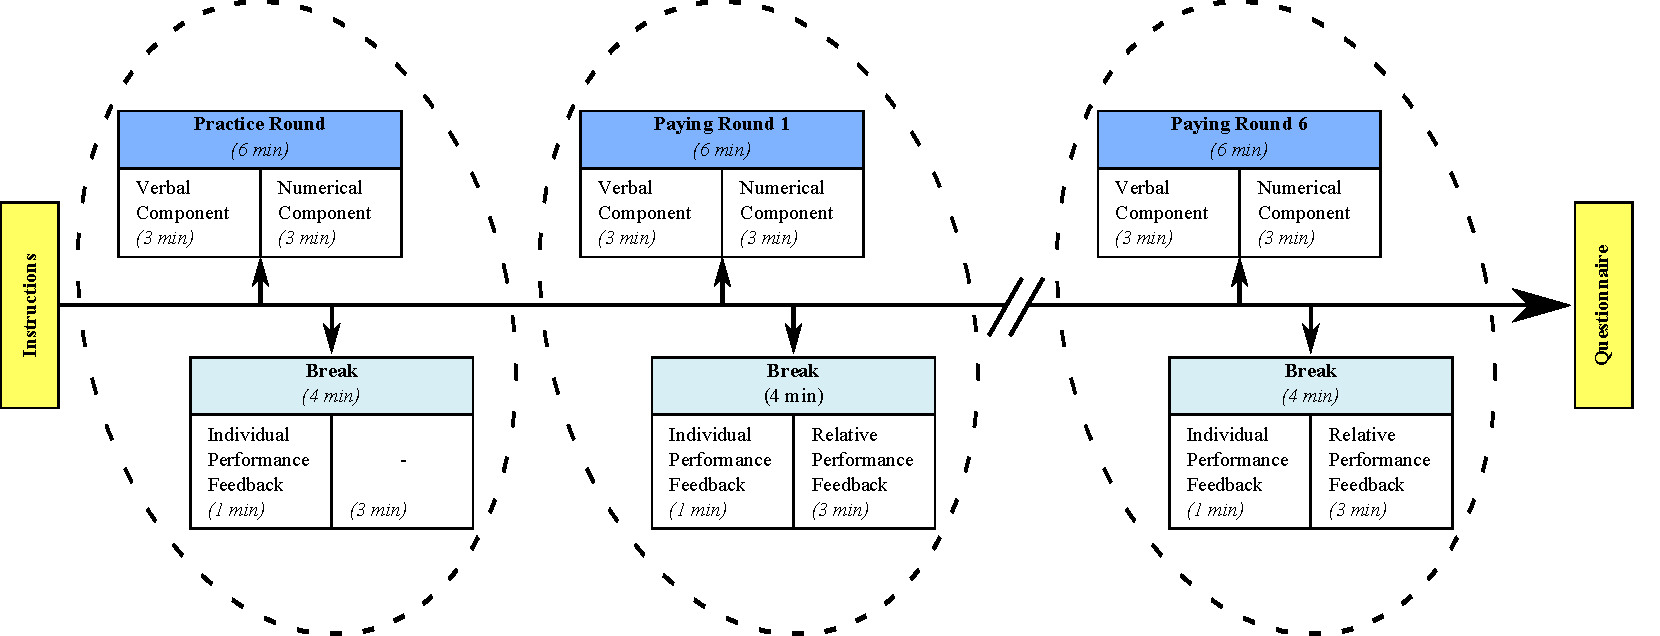
\includegraphics[width=\linewidth]{images/fig1-4.pdf}
    \caption{The stages and the timing of the experiment.}
    \label{fig:experiment-stages}
  \end{center}      
\end{figure}
\vspace{-2em}
\section{Introduction}
Currently at version 0.7.4, the \emph{Gender-Neutral Real-Effort Task} (GNRET) is a collection of individual feedback driven end-user tasks and a master control application to monitor the ongoing experiment in real-time from a remote location. Under the supervision of Dr.~Victoria Prowse, this study was designed by Zdenka Kissov\'{a} as a partial fulfillment of the requirements for the degree of M.Phil.~in Economics at University of Oxford. The experiments were conducted in the experimental laboratory of the Nuffield Centre for Experimental Social Sciences (CESS) at University of Oxford. The actual software was delivered by Jozef Dobo\v{s} from the Department of Computer Science, University College London.
	
		
The executable with the corresponding \emph{change log} can be found at a password protected online storage location: \url{http://www.jozef.xn--dobo-j6a.eu/media/zdenka/}.

\section{Program Flow}
\autoref{fig:experiment-stages} outlines the stages and timing of the experiment. Each experimental session lasts for approximately 90 minutes and consists of seven (one practice and six paying) 6-minute rounds. In
each 6-minute round, the initial 3 minutes are allocated to the verbal component of the task (word spotting), followed by another 3 minutes of numerical questions (adding up) all of which are automatically timed out. There is a 4-minute break after each round. During the first minute of this break, participants can always see their
individual total points score (the sum of the verbal and numerical point scores) for the respective round on their screens. In the last three minutes of the break, Treatment Group subjects receive treatment-specific relative performance feedback. The demographics and behavioural data questionnaire is displayed after the last experimental round. The questionnaire asks about basic demographics such as gender, age, country of origin and degree of study as well as the subject's perceived level of competitiveness, familiarity with the task, satisfaction with the performance and the potential use of performance goals.


\begin{figure}[!tb]
  \begin{center}
  	\subfigure[Word Spotting Task] {
    	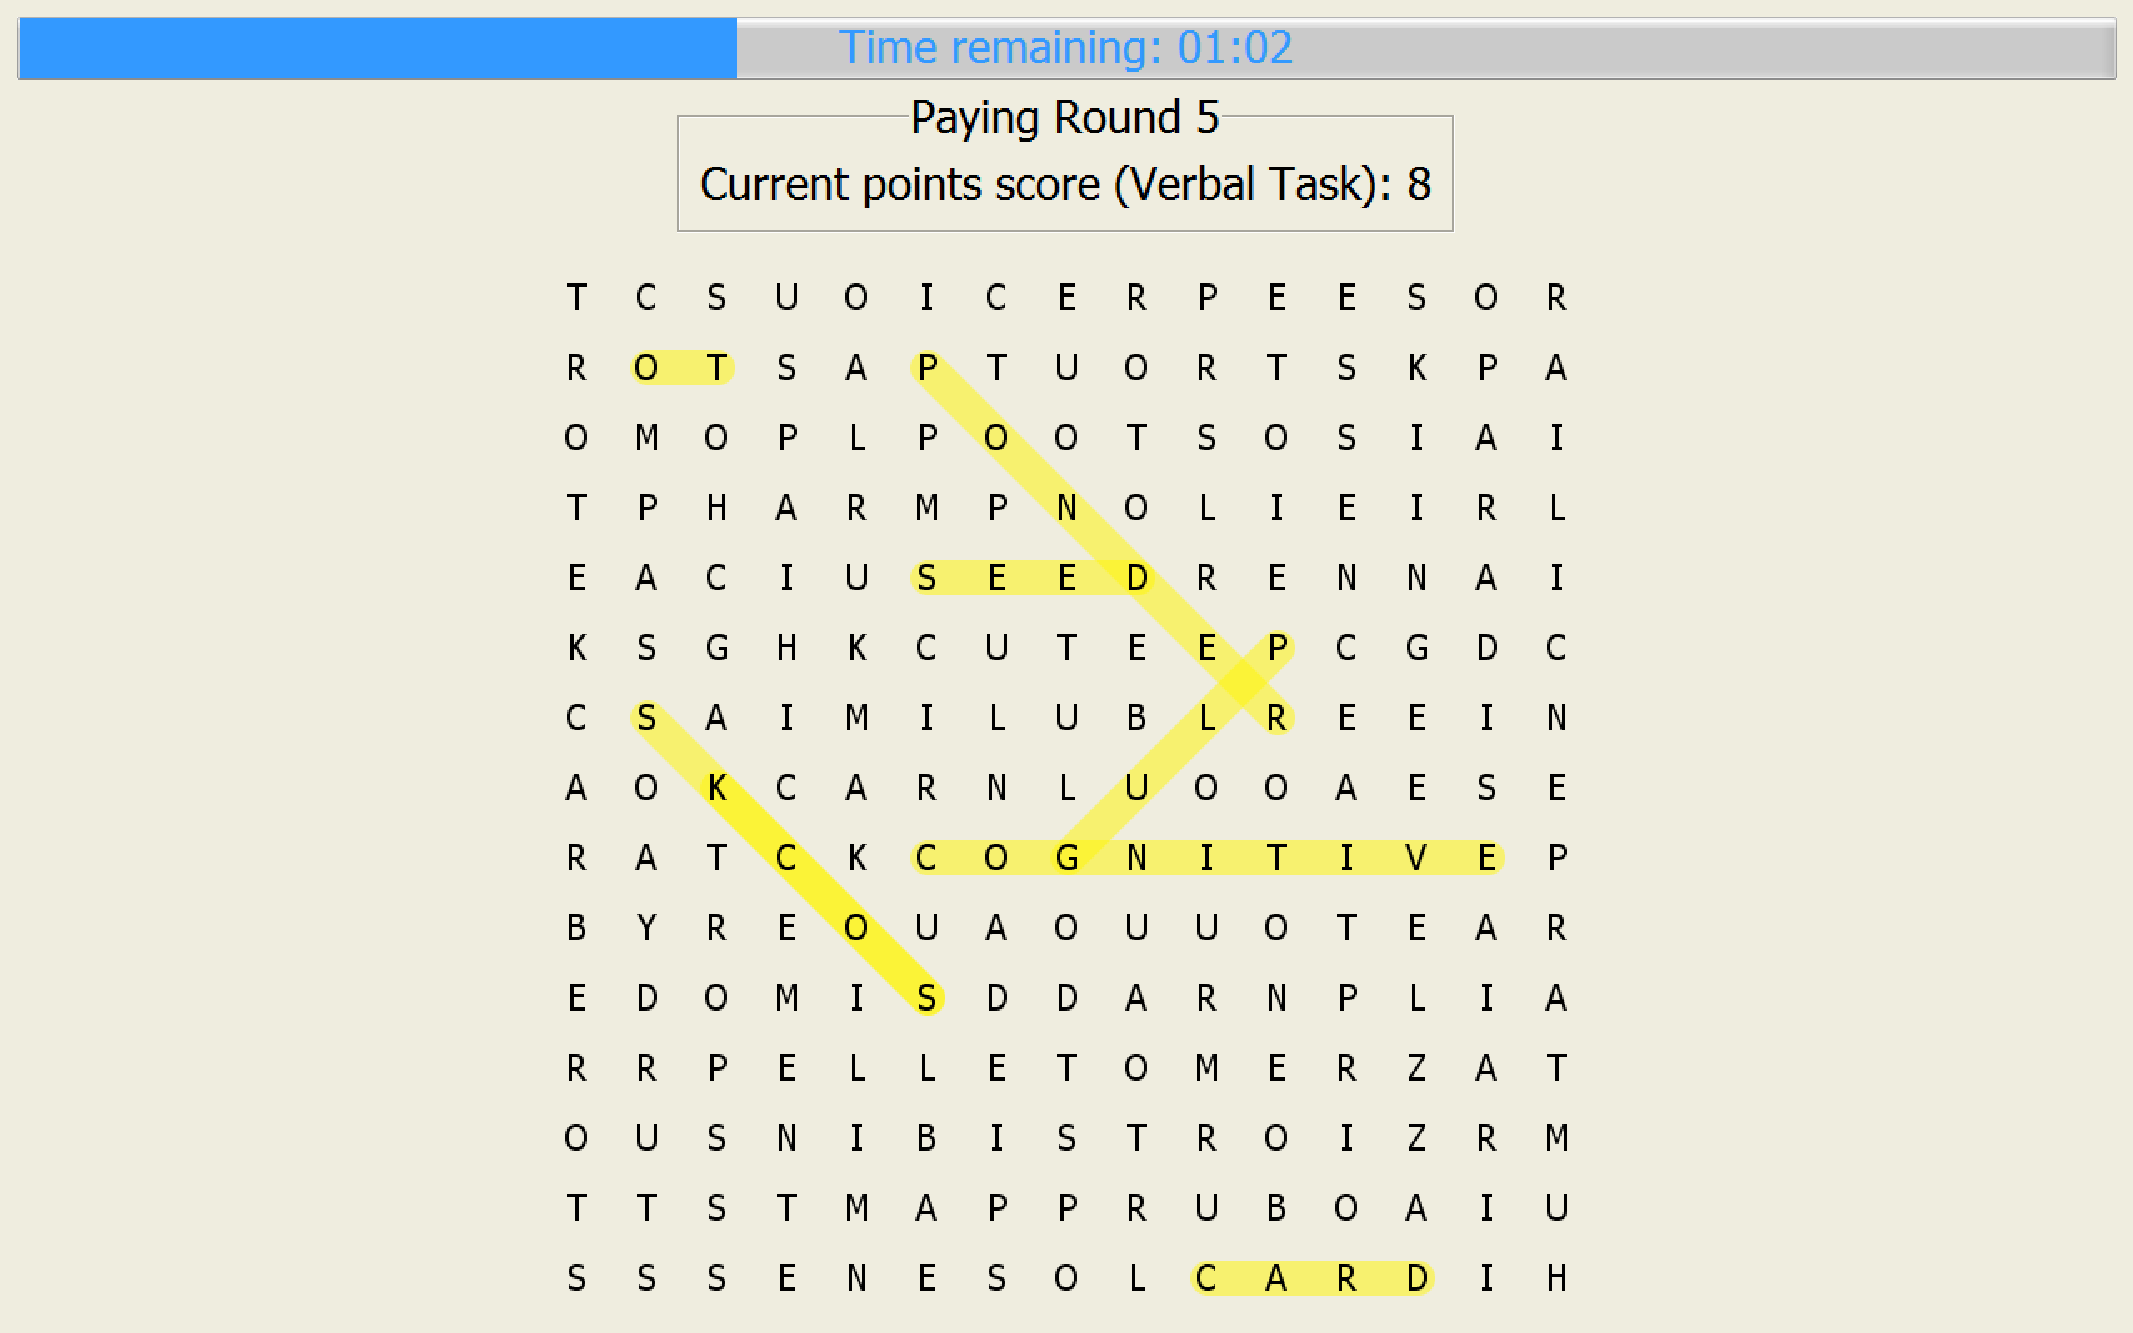
\includegraphics[width=0.48\linewidth]{images/verbal.pdf}
    	\label{word-spotting-task}
    }
    \subfigure[Numerical Task] {
    	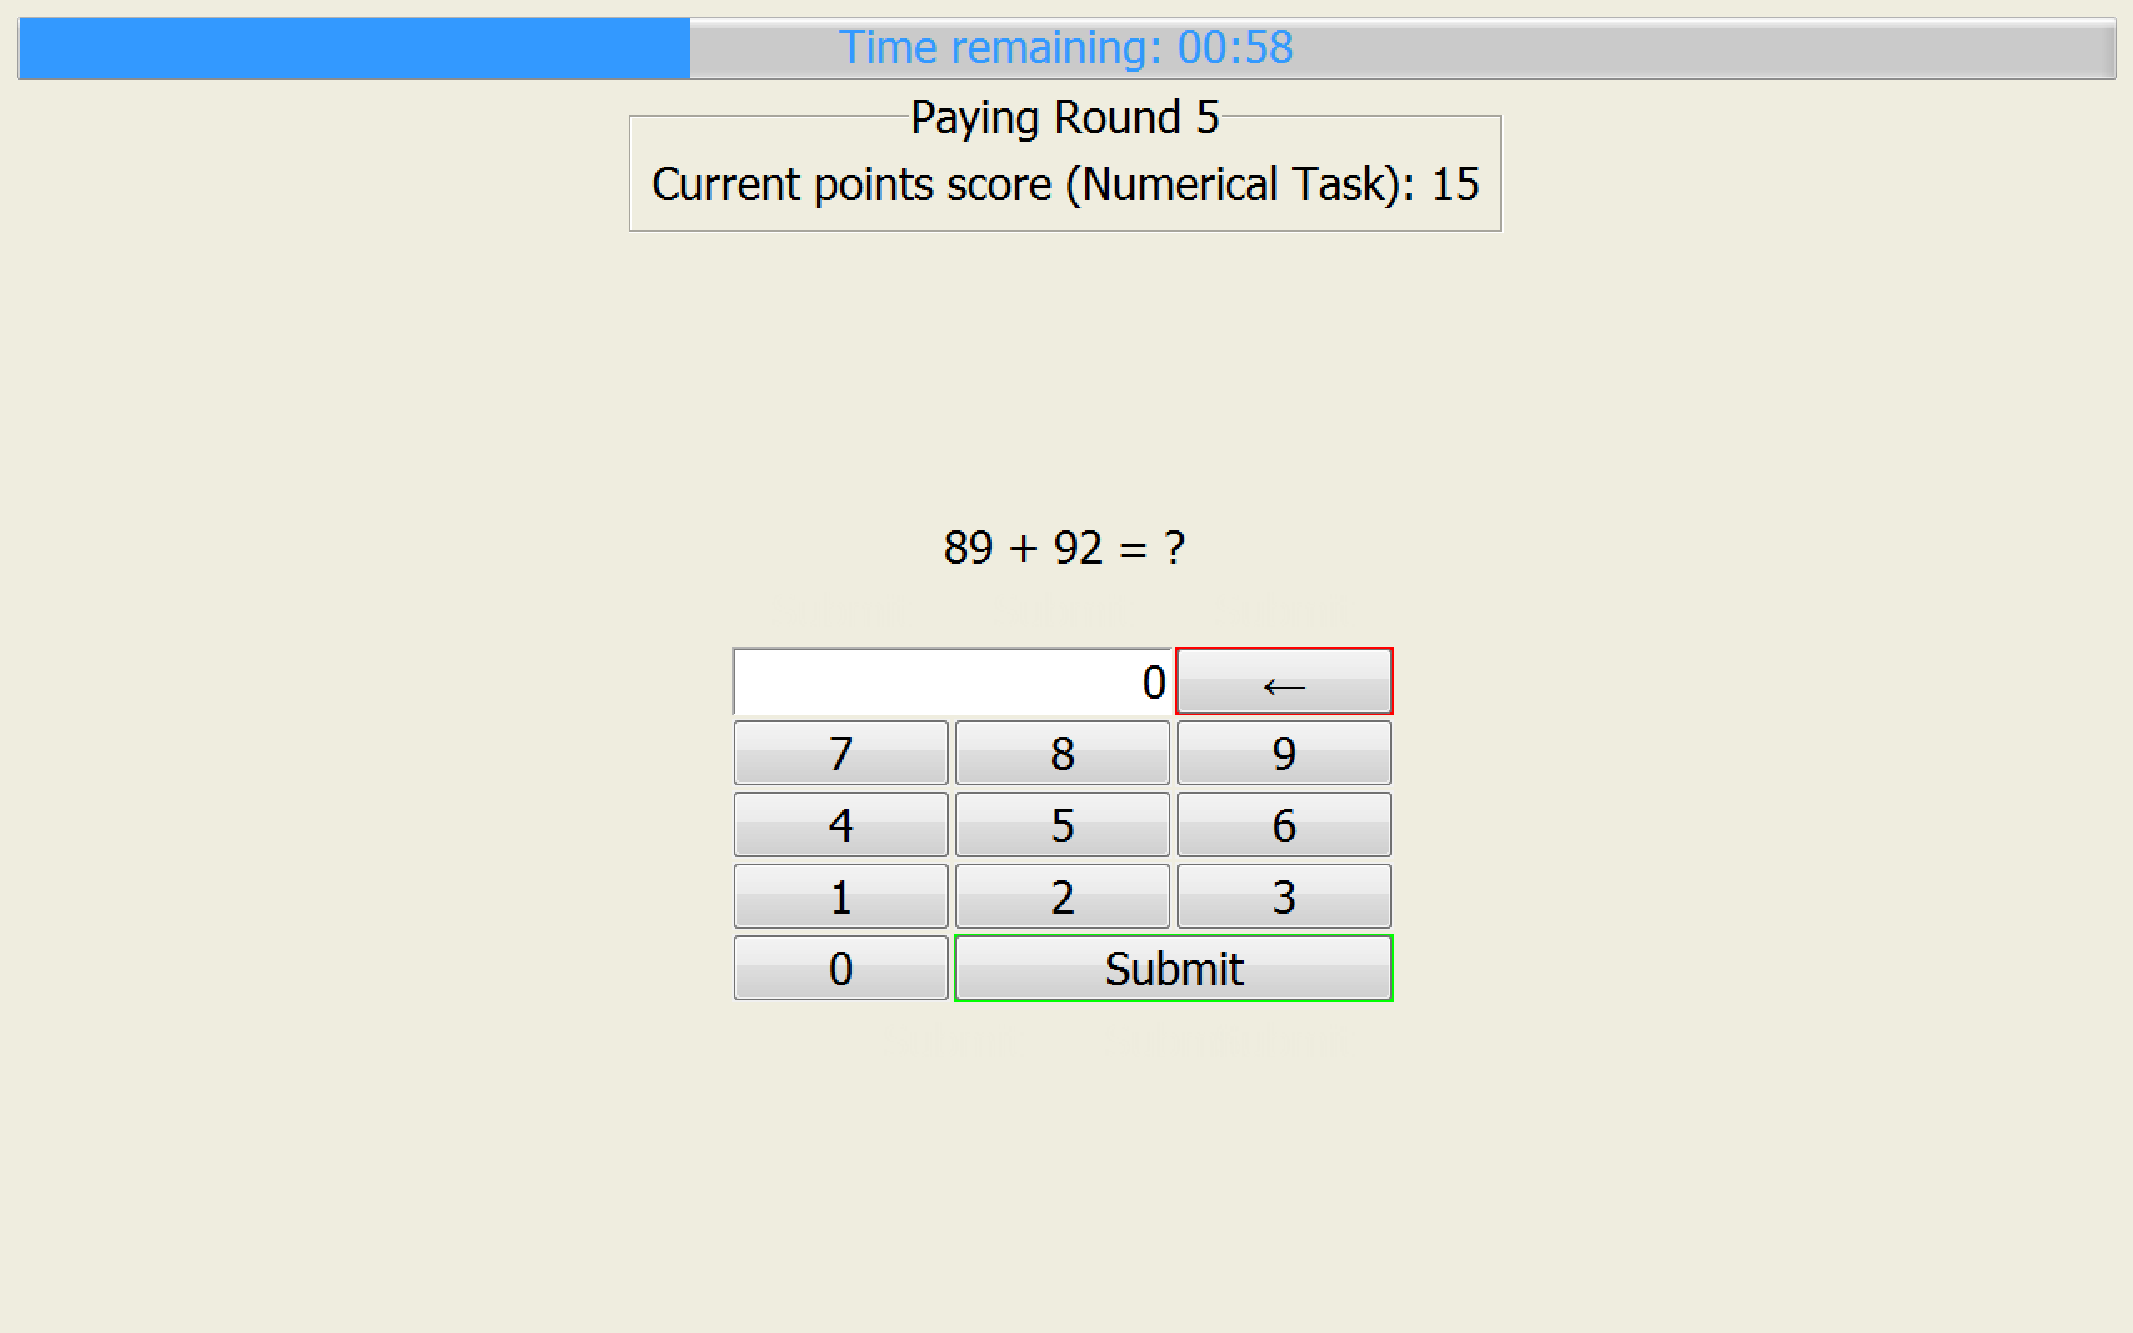
\includegraphics[width=0.48\linewidth]{images/numerical.pdf}
    	\label{numerical-task}
    }
  \end{center}   
    \caption{(a) The letter grid for word spotting used in the Practice Round across all sessions. (b) The numerical grid with an adding up question used in the Practice Round across all sessions.}
  \end{figure}
  

\subsection{Word Spotting Task}

During the word spotting, each subject is presented with a 15 by 15 grid of capital letters, see Figure \autoref{word-spotting-task}, and is asked to look for English words in horizontal, vertical or diagonal direction, forward or backward. A word is selected using the mouse.\footnote{This ensures that the subjects are not disadvantaged based on their typing skills.} The subjects need to place the cursor of the mouse over the starting letter of a proposed word, pull the cursor to the last letter of that word and then release the cursor.\footnote{The first and last letter recognition prevents pure guessing.} If the selected word is valid, it remains highlighted and a point is awarded. No points are awarded or subtracted for incorrect entries so as to avoid potential hostile framing or punishment effects in the subjects' behaviour.


\subsection{Numerical Task}
After the initial three minutes elapse, an adding up question for a pair of 2-digit numbers automatically appear on the screen. The subject needs to correctly sum the numbers to win a point and proceed to the next numerical question. Calculators, pens and paper are not allowed. The answer is entered using the mouse and a calculator-style number pad on the screen. As in
the verbal component of the task, no points are awarded or subtracted for incorrect entries. The points from the verbal and numerical task components in a specific round are added up to form the total point score for that round. Identical letter grids and number questions in the same order are used across all sessions and hence all treatment groups.


\begin{figure}[hbt]
  \begin{center}
  	\subfigure[Individual Performance Feedback] {
    	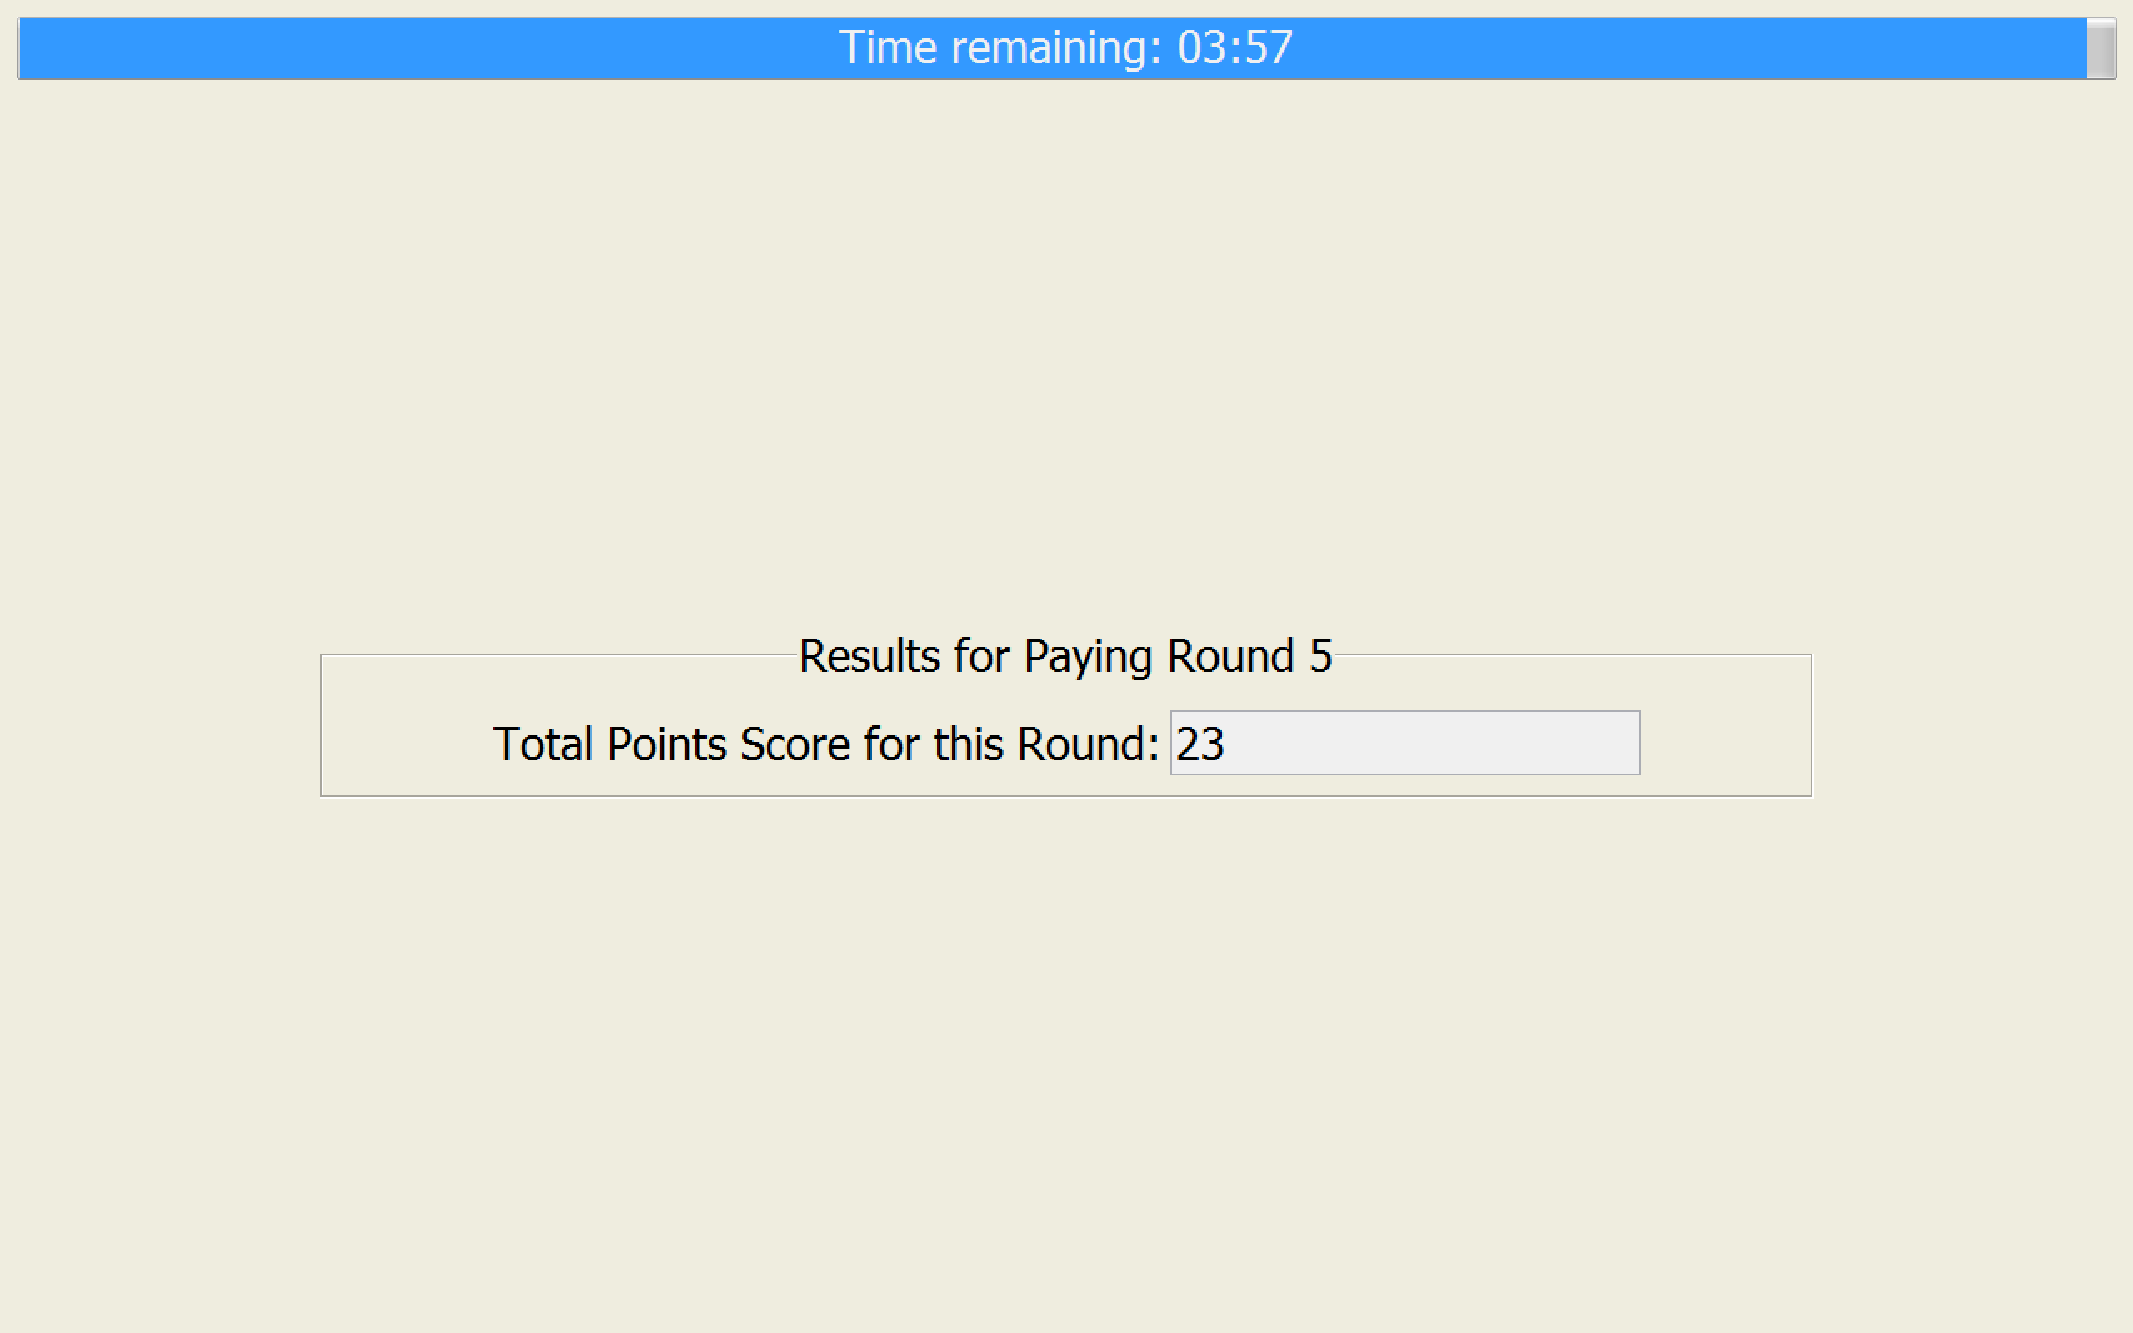
\includegraphics[width=0.48\linewidth]{images/score.pdf}
    }
    \subfigure[Relative Performance Feedback] {
    	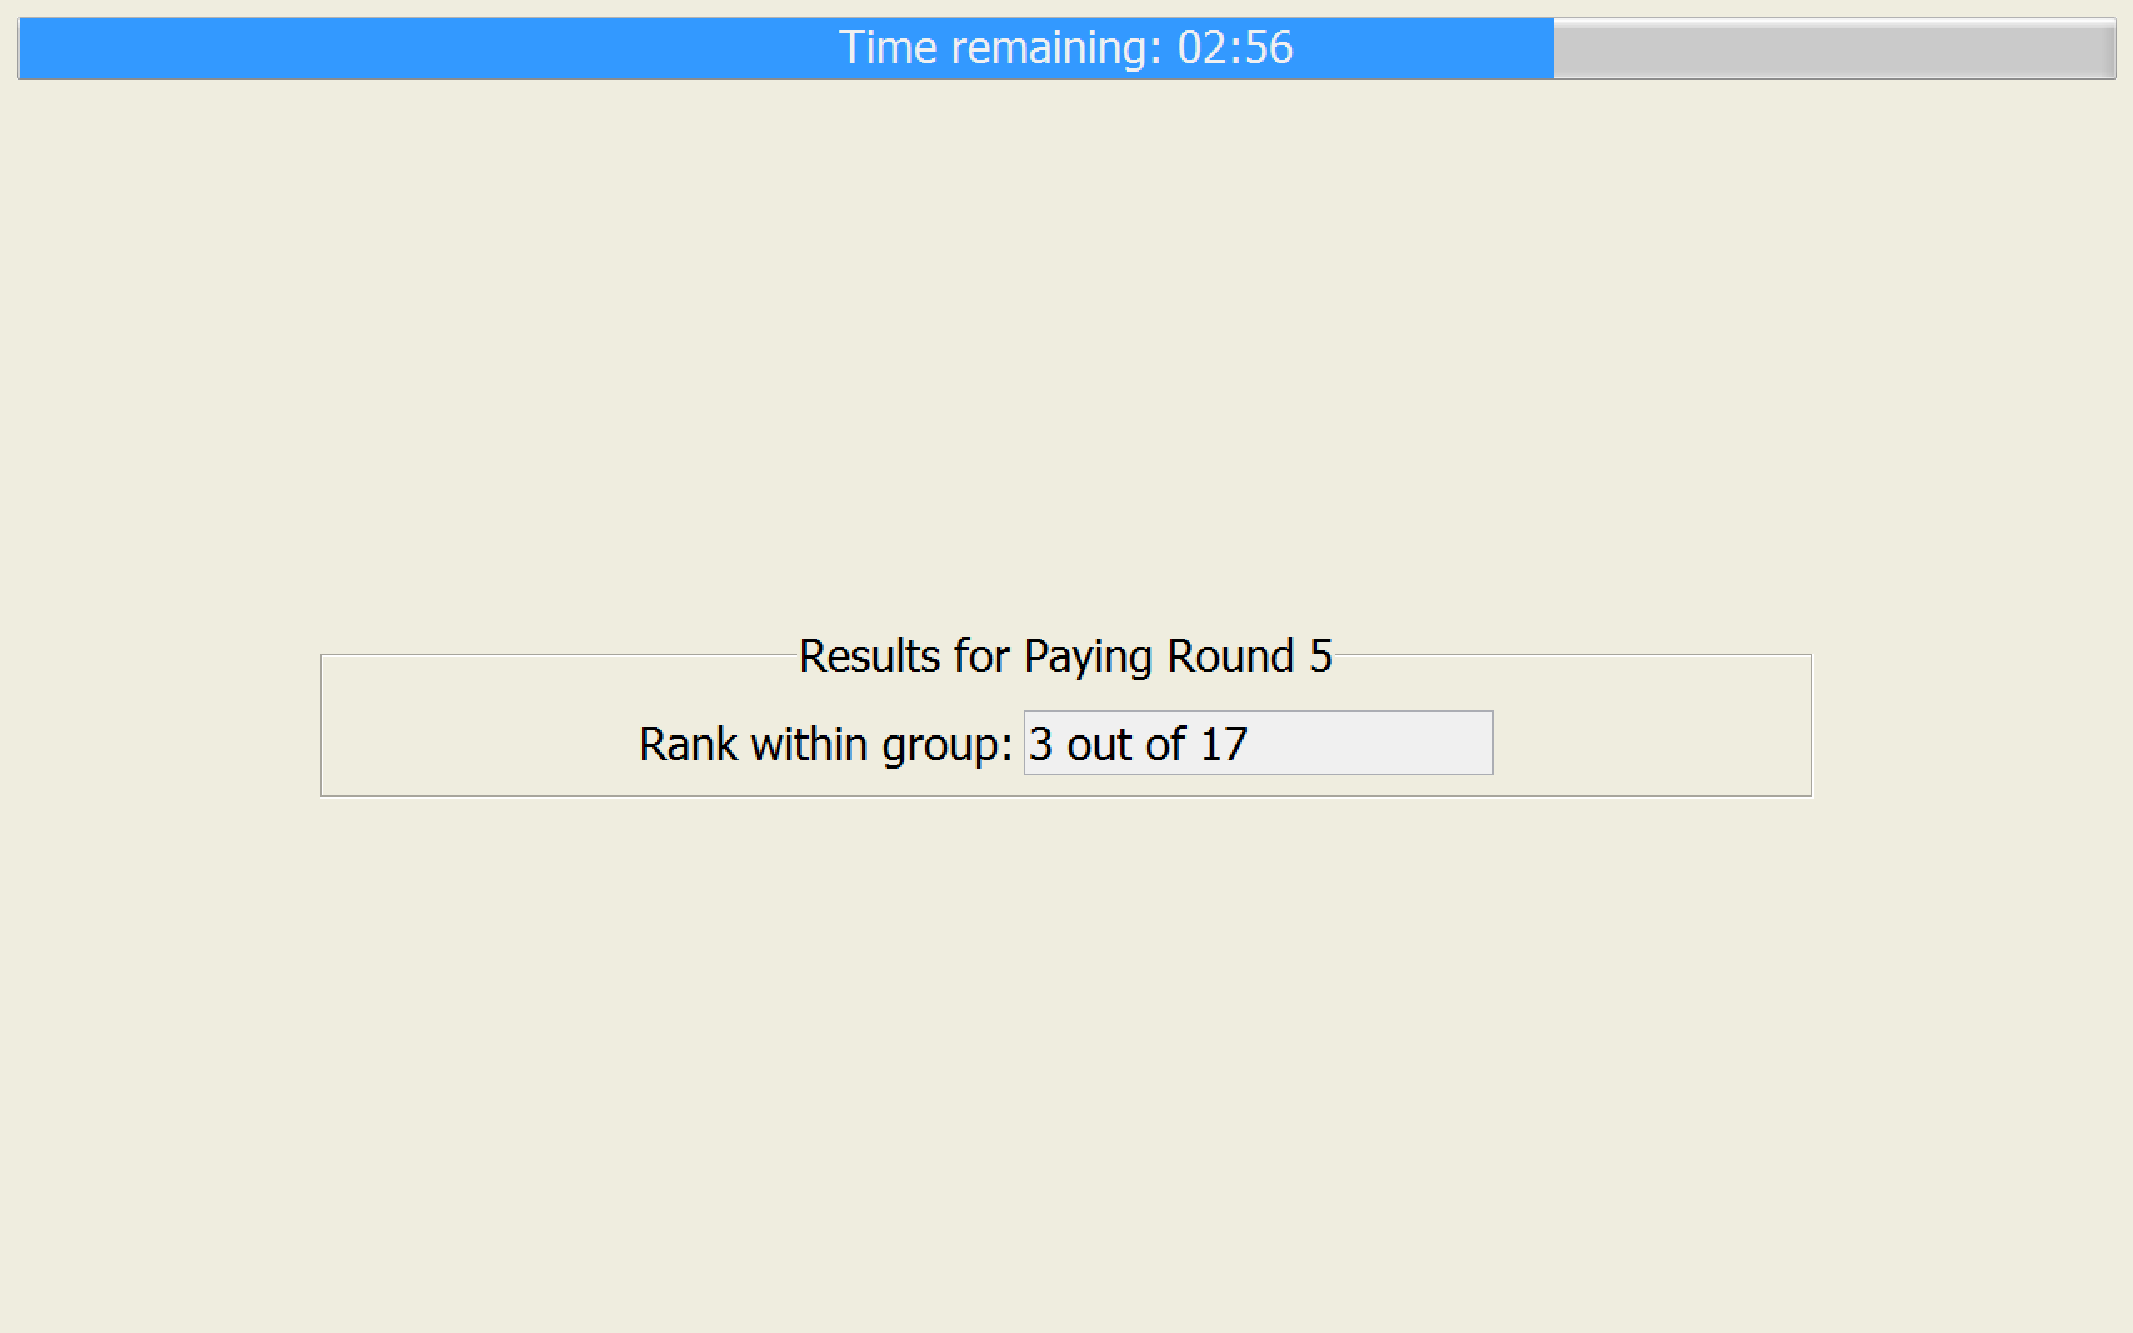
\includegraphics[width=0.48\linewidth]{images/rank.pdf}
    }
    
    \caption{Individual and relative performance feedback as displayed during (a) the first and (b) the last three minutes of the break to Treatment Group 1. Note that the first-minute individual performance feedback was displayed in the same manner to all subjects across the experiment.}
    
  \end{center} 
  \label{fig:score-and-rank}
  \end{figure}
  

\subsection{Performance Feedback}
Subjects are divided into four groups with the same selection and order of the tasks, but with different performance feedback as follows:
\begin{itemize}
	\item {\bfseries Control Group (C)} -- no relative performance feedback.
	\item {\bfseries Treatment Group 1 (T1)} -- computerised private relative performance feedback.
	\item {\bfseries Treatment Group 2 (T2)} -- personal private relative performance feedback.
	\item {\bfseries Treatment Group 3 (T3)} -- personal public relative performance feedback.
\end{itemize}

	
%\begin{figure}[thbp]
%	\centering
%  \includegraphics[width=\linewidth]{images/bem.pdf}
%  \caption{Courtesy of Arup.}
%  \label{fig:bem}
%\end{figure}

\section{Technical Information}

The front-end Graphical User Interface (GUI) is written in Java Swing with networking provided by the Apache Commons library executed in an exclusive full-screen mode to avoid any unnecessary distractions.


\begin{wrapfigure}{r}{0.25\linewidth}
\vspace{-28pt}
\begin{center}
  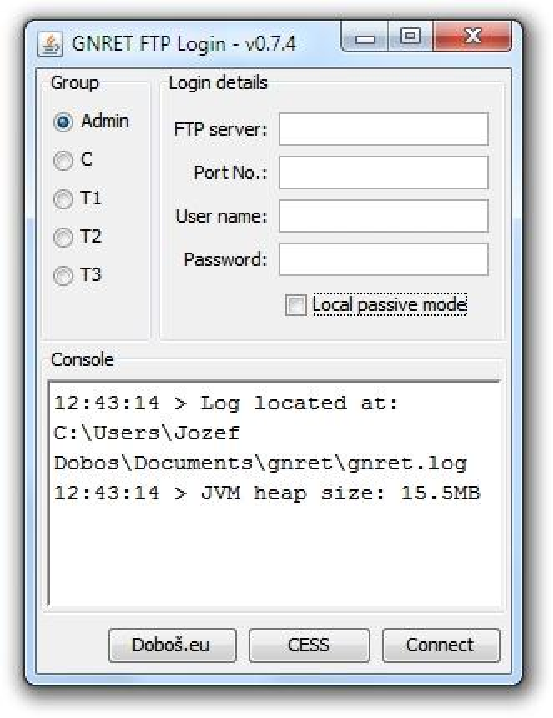
\includegraphics[width=\linewidth]{images/login.pdf}
  \caption{FTP Login window showing location of the log file.}
   \label{applab}  
  \end{center}  
  \vspace{-26pt}
\end{wrapfigure}


Once started, each \emph{client} application, the one that the subjects interact with, opens up a File Transfer Protocol (FTP) connection to the master server from which it polls for a start and every round signals triggered by the \emph{admin interface}. Only if the corresponding buttons are set, see \autoref{fig:admin} for toolbar options, will the individual sections as outlined in \autoref{fig:experiment-stages} automatically proceed. Client saves locally a text file with all so far collected responses which is uploaded to the main FTP server during each break. Admin program automatically calculates the rank of each client and saves the results to the FTP server from which the client if in T1 mode requests this information and displays it on the screen. Intermediate results as well as the final questionnaire answers are viewable in the admin interface. 

\subsection{Error Handling}

In the case of crash, there is always a local copy of the subject's responses as well as a program log file. If the FTP connection is dropped, the client will automatically attempt reconnection with a randomised interval of 30 to 60 seconds in between as to prevent overloading the server.




\begin{figure}[!htb]
  \begin{center}
    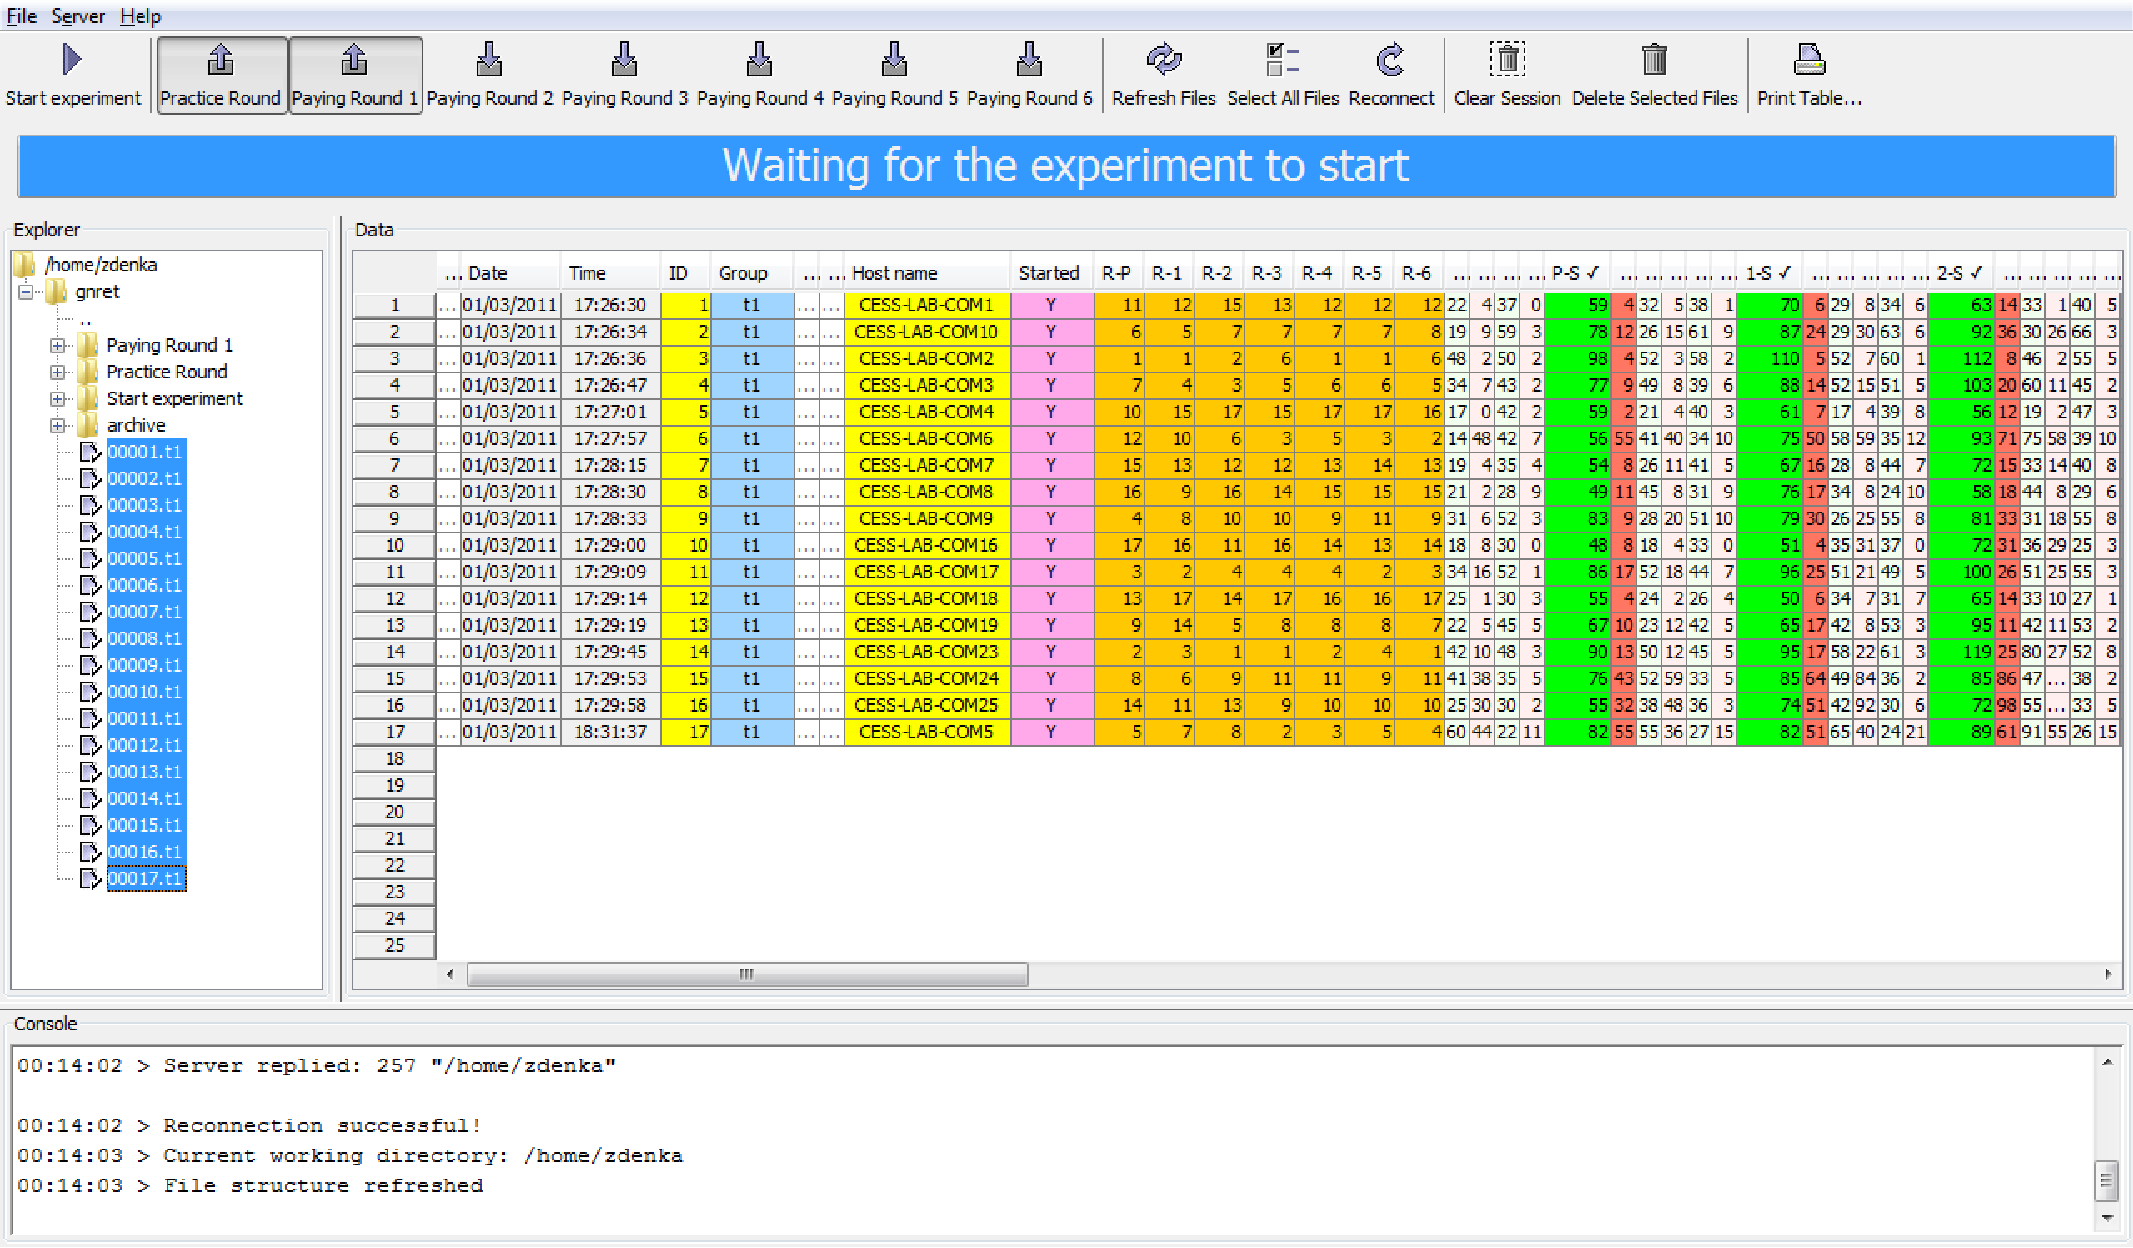
\includegraphics[width=\linewidth]{images/admin.pdf}
    \caption{Admin interface for live monitoring of the experiment.}
      \label{fig:admin}
  \end{center}  
\end{figure}


\subsection{Requirements}
\begin{itemize}
 \item \emph{Java Runtime Environment} v1.4+.
 \item \emph{Java Webstart} plugin.
 \item \emph{MS Windows} or \emph{Linux} based FTP server with password protected write access.
\end{itemize}
Downloadable from \url{http://www.java.com/en/download/index.jsp}.

\subsection{External Dependencies}

\begin{description}
	\item[Apache Commons Net 2.2.] This standard Apache release library provides networking functionality through FTP and socket connection wrappers and is distributed under the \emph{Apache License Version 2.0} (January 2004), can be found at: \url{http://www.apache.org/licenses/}.
	
	\item[Java File Graphics 1.0.] Former Sun Microsystems created a standard icon graphics library to distribute with their Java Swing applications.
	
	\item[Jazzy Core Spell Checker.] Jazzy Core implements spell checking algorithm similar to \emph{aspell} and is distributed under \emph{GNU Lesser General Public License Version 2.1} (February 1999). The source and precompiled libraries can be found at: \url{http://sourceforge.net/projects/jazzy}.
	
	\item[ISpell Word Lists.] A word list compiled from American and British English spelling lists of the \emph{Ispell Version 3.1.20} distributed under a royalty free license, a copyright 1993 of Geoff Kuenning, Granada Hills, CA, USA. The individual dictionaries can be found at: \url{http://wordlist.sourceforge.net/}.
\end{description}



\end{document}

